\chapter{Simulazione}
Per valutare le prestazioni del sistema realizzato si sono effettuate numerose simulazioni. Tutti i test condotti sono stati basati su una specifica configurazione di nodi, in particolare 1 nodo Publisher e 2 Subscriber. I due nodi consumer richiedono la stipulazione di un contratto al producer, il quale espleta tutte le richieste. Si riporta ora un esempio di esecuzione con relativa descrizione ed analisi dei dati.
\section{Esecuzione}
In principio si avvia il nodo Producer il quale andrà in attesa di richieste dei consumatori. In seguito si avviano i due Consumer (o Subscriber) i quali richiedono ed ottengono un contratto con il Subscriber. Stabiliti i contratti inizia la vera fase di simulazione in cui ogni nodo genera valori casuali per le proprie risorse e lo SC raccoglie tali dati per valutare gli SLA e la necessità di migrazione. Per eseguire il sistema bisogna utilizzare i seguenti comandi;
\begin{verbatim}
ant runGui
\end{verbatim}
per avviare il \code{MainContainer}
\begin{verbatim}
ant -f build2.xml AgentLauncher
\end{verbatim}
che avvia i tre nodi in tre container differenti.
\subsection{Scenario}
I tre nodi dello scenario d'esecuzione hanno le seguenti caratteristiche:
\begin{enumerate}
	\item Publisher con connessione WIRED e 512Kb di banda;
	\item subscriber con connessione WIRELESS e 256Kb di banda;
	\item subscriber con connessione WIRELESS e 256Kb di banda.
\end{enumerate}
\subsection{Generazione contratti SLA}
Il contratto SLA, ovvero i livelli di latency, reliability e reqInterval vengono generati casualmente dal publisher nel momento in cui raccolgono una richiesta di contratto. Tale operazione può essere vista nel log di esecuzione del programma simulativo.
\begin{enumerate}
\item Il Subscriber richiede un contratto con un qualsiasi publisher disponibile;
\item Il publisher legge la richiesta dal dsm;
\begin{center}
\begin{verbatim}
SLAContract-request received from cm2
\end{verbatim}
\end{center}
\item il publisher genera i parametri del contratto casualmente e lo immette sul dsm;
\item lo SC rileva la presenza del contratto e lo aggiunge alla sua lista.
\begin{center}
\begin{verbatim}
Added Contract
\end{verbatim}
\end{center}
\end{enumerate}
\subsection{Migrazione}
Inizialmente lo SC risiede sul primo nodo, ovvero il publisher (ved. \ref{fig:primo}).
\begin{figure}[H]
\begin{center}
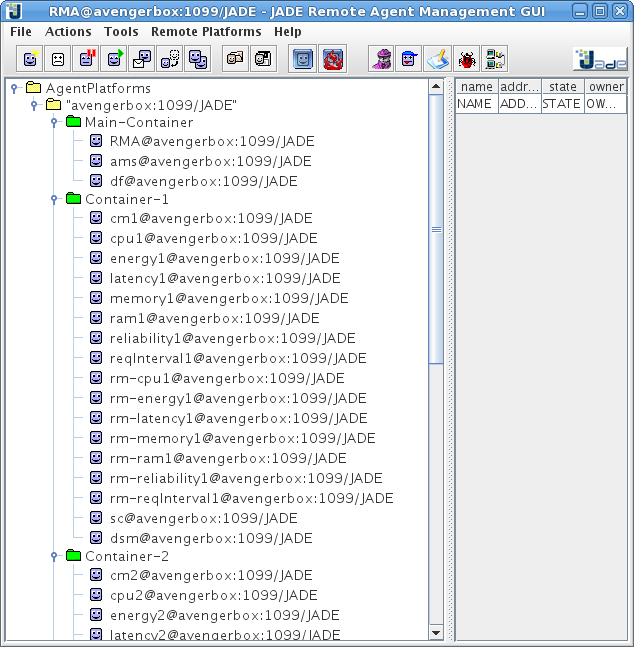
\includegraphics[scale=0.5]{etc/primo.png}
\caption{Migrazione non avvenuta}
\label{fig:primo}
\end{center}
\end{figure}
In questa figura si può notare la presenza del dsm e dello SC sul primo nodo, in quanto la simulazione è stata appena avviata. Dal log si può rilevare che lo SC ha già iniziato a controllare la necessità di migrazione e che al momento si trova sul Container-1 ovvero il nodo 1. Il valore index del nodo attuale non ha ancora superato il valore di soglia (52), di conseguenza lo SC rimane sul nodo attuale.
\begin{lstlisting}
Sono su Container-1
Context[cm3]--> cpu: 40.092556, ram: 16.937687, memory: 34.849556, energy: 81.61731, index: 26.647161
Context[cm1]--> cpu: 57.77024, ram: 51.60415, memory: 45.732647, energy: 100.0, index: 35.674618
Context[cm2]--> cpu: 4.5756726, ram: 52.93144, memory: 40.222347, energy: 98.34838, index: 22.97326
Associated with: cm1
Actual context--> cpu: 57.77024, ram: 51.60415, memory: 45.732647, energy: 100.0, index: 35.674618
\end{lstlisting}
Nel momento in cui il carico su tale nodo raggiunge valori troppo alti avverrà la migrazione. Infatti poco tempo dopo si ha una situazione del genere:
\begin{lstlisting}
Sono su Container-1
Context[cm3]--> cpu: 10.354793, ram: 26.346369, memory: 2.7747908, energy: 75.6174, index: 16.394249
Context[cm1]--> cpu: 77.09479, ram: 64.88432, memory: 87.20903, energy: 100.0, index: 52.713272
Context[cm2]--> cpu: 5.725228, ram: 59.014675, memory: 7.089407, energy: 92.148476, index: 18.876198
Associated with: cm1
Actual context--> cpu: 77.09479, ram: 64.88432, memory: 87.20903, energy: 100.0, index: <52.713272>
Migration to cm3
Moving DSM to 3

Sono su Container-3
Context[cm1]--> cpu: 7.0192904, ram: 18.302485, memory: 86.83973, energy: 100.0, index: 25.797146
Context[cm2]--> cpu: 25.42843, ram: 30.698774, memory: 4.063858, energy: 91.34849, index: 16.4394
Context[cm3]--> cpu: 3.4131508, ram: 16.183126, memory: 7.618082, energy: 74.61742, index: 13.874079
Associated with: cm3
Actual context--> cpu: 3.4131508, ram: 16.183126, memory: 7.618082, energy: 74.61742, index: <13.874079>
\end{lstlisting}
l'indice sul nodo attuale ha raggiunto un valore di 57.71 a causa di un elevato uso delle risorse disponibili, in particolare della della memoria. Dalla figura \ref{fig:secondo} si può notare che il dsm e lo SC si sono spostati sul Container-3. Su quest'ultimo nodo l'indice è adesso di 21.1.
\begin{figure}[H]
\begin{center}
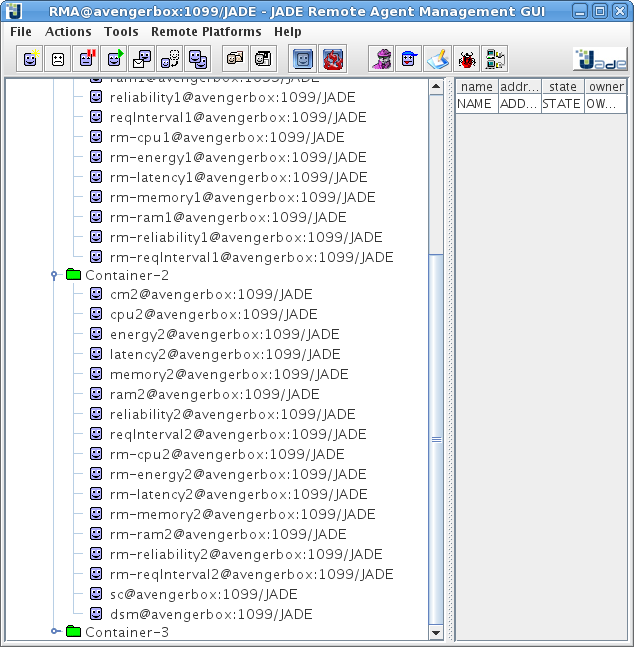
\includegraphics[scale=0.5]{etc/secondo.png}
\caption{Migrazione su secondo nodo}
\label{fig:secondo}
\end{center}
\end{figure}
Il nodo 3 è di tipo WIRELESS e quindi ha una energia limitata, il che implica un tempo di residenza per l'SC e il dsm molto più ridotto, in quanto l'indice raggiungerà rapidamente valori alti.
\begin{lstlisting}
Sono su Container-3
Context[cm1]--> cpu: 0.81155604, ram: 33.999382, memory: 51.11227, energy: 100.0, index: 19.762337
Context[cm2]--> cpu: 36.432972, ram: 58.424694, memory: 1.620206, energy: 84.948586, index: 26.705338
Context[cm3]--> cpu: 67.67117, ram: 95.22946, memory: 26.253895, energy: 49.21744, index: 58.74031
Associated with: cm3
Actual context--> cpu: 67.67117, ram: 95.22946, memory: 26.253895, energy: 49.21744, index: <58.74031>
Migration to cm1
Moving DSM to 1

Sono su Container-1
Context[cm1]--> cpu: 50.261562, ram: 62.669903, memory: 48.456142, energy: 100.0, index: 37.11915
Context[cm2]--> cpu: 1.1113803, ram: 6.8676476, memory: 18.00424, energy: 83.9486, index: 10.791573
Context[cm3]--> cpu: 83.216156, ram: 71.41142, memory: 32.01974, energy: 44.21744, index: 59.663654
Associated with: cm1
Actual context--> cpu: 50.261562, ram: 62.669903, memory: 48.456142, energy: 100.0, index: <37.11915>
\end{lstlisting}
L'energia del nodo 3 è scesa da 49 a 44 il che ha costretto la migrazione sul nodo meno carico, ovvero l'uno (WIRED). In seguito vi è stata anche una violazione del contratto ed è stata segnalata ad entrambi i nodi partecipanti al contratto, i quali dovranno adattarsi per evitare di ripetere la violazione.
\begin{lstlisting}
Violated with latency 23.106468 > 82.419365, reliability 41.978447 > 99.44324, reqInterval 79.21008 > 76.23332
\end{lstlisting}
Dal log si può notare che è stato il subscriber ad eccedere in rischieste, infatti il reqInterval è inteso come frequenza.
\section{Analisi dati}
In questa sezione verranno esposti e commentati i grafici relativi alla simulazione, in quanto molto più esplicativi dei log riportati sopra. Tutti i grafici riportati avranno come ascisse i secondi che non rappresentato un valore reale ma simulato, infatti servono per dare un senso più reale alla simulazione. 
\subsection{Indice}
L'indice è il valore più importante del test eseguito, in quanto la migrazione si basa su di esso. Come passo fondamentale vengono ora riportati i grafici relativi agli indici.
\begin{figure}[H]
\begin{center}
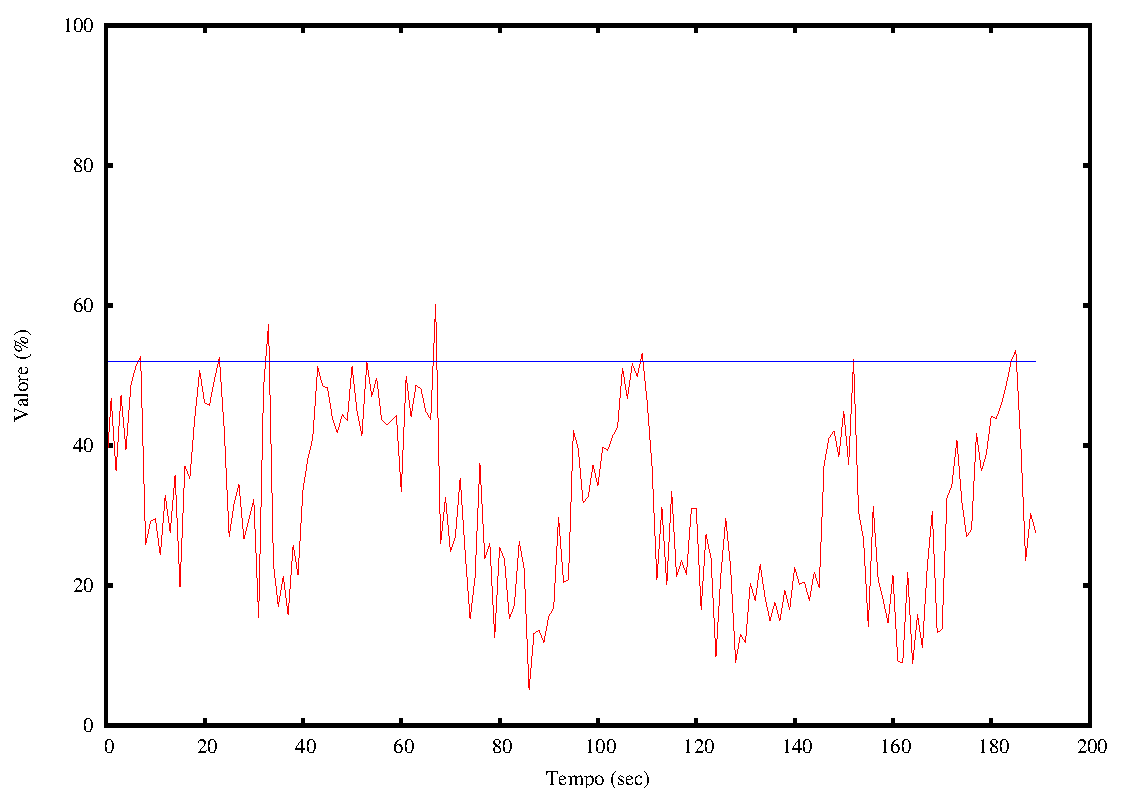
\includegraphics[scale=0.6]{etc/index1.pdf}
\caption{Indice primo nodo}
\label{fig:index1}
\end{center}
\end{figure}
\begin{figure}[H]
\begin{center}
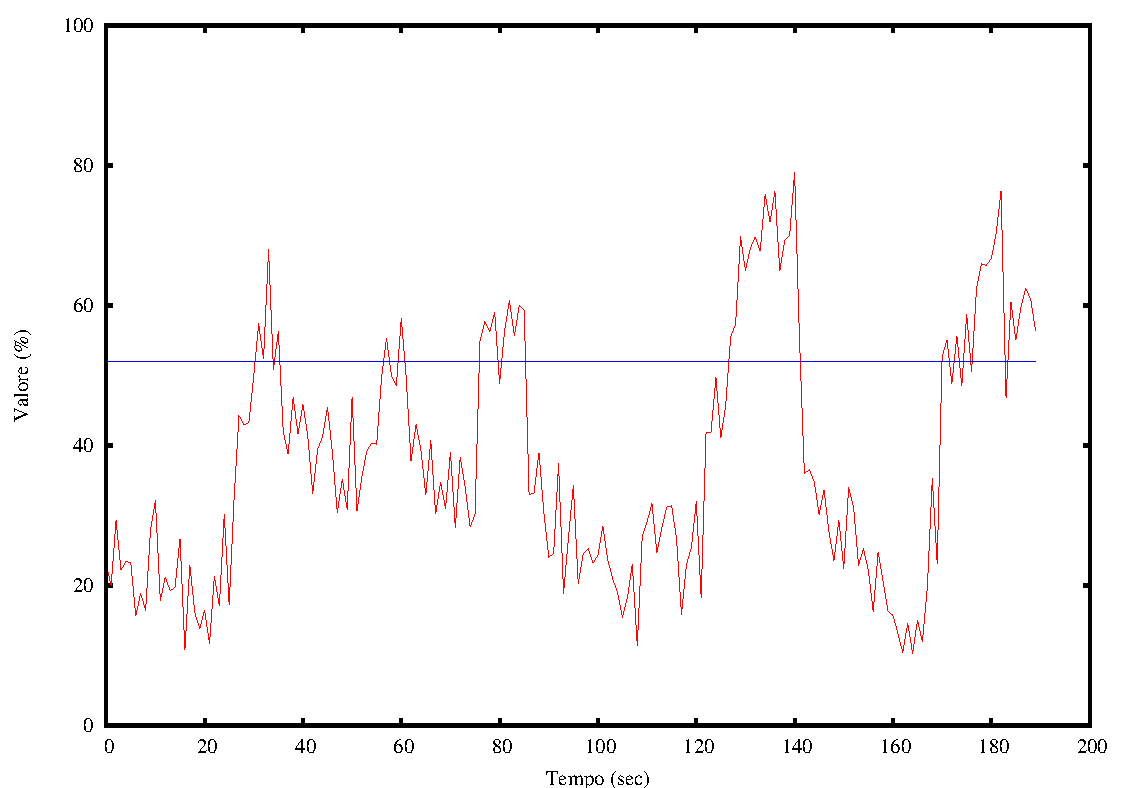
\includegraphics[scale=0.6]{etc/index2.pdf}
\caption{Indice secondo nodo}
\label{fig:index2}
\end{center}
\end{figure}
\begin{figure}[H]
\begin{center}
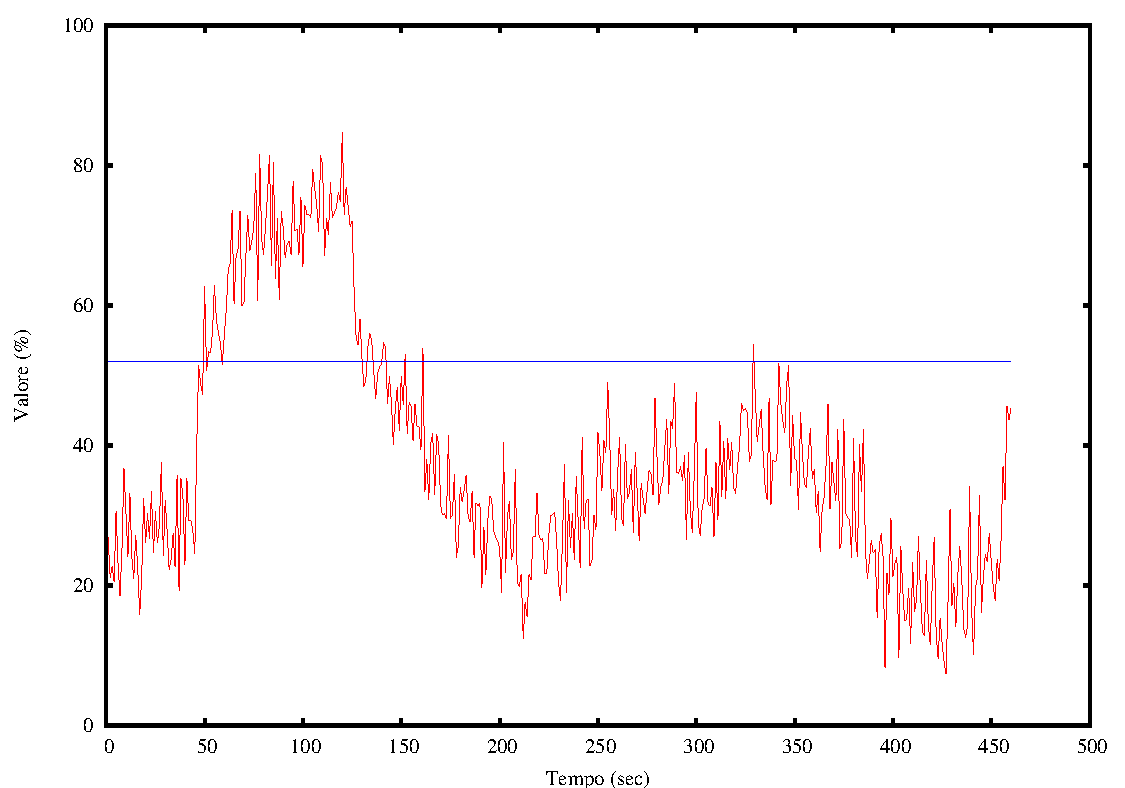
\includegraphics[scale=0.6]{etc/index3.pdf}
\caption{Indice terzo nodo}
\label{fig:index3}
\end{center}
\end{figure}
\begin{figure}[H]
\begin{center}
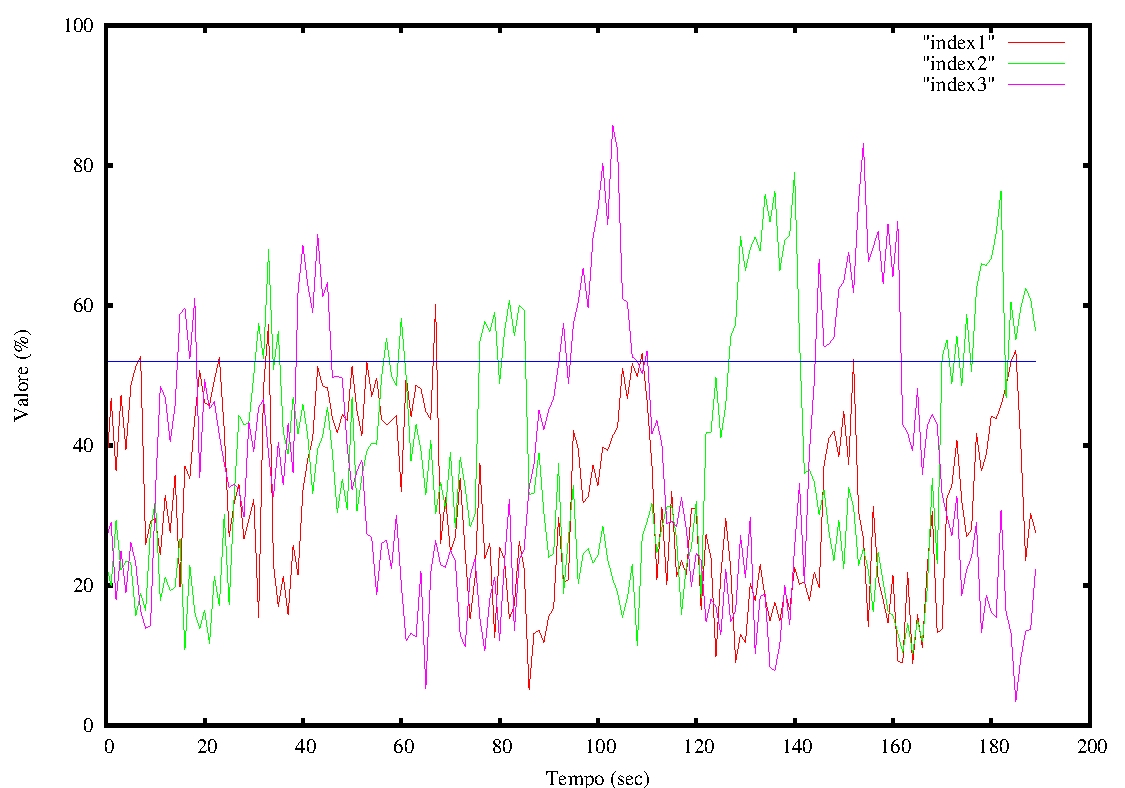
\includegraphics[scale=0.6]{etc/index.pdf}
\caption{Indice tutti i nodi}
\label{fig:index}
\end{center}
\end{figure}
Nelle figure \ref{fig:index1}, \ref{fig:index2}, \ref{fig:index3} e \ref{fig:index} si può notare la presenza di una retta di colore blu, questa rappresenta il limite dell'indice, ovvero 52. Per comprendere meglio i grafici basta sapere che quando i punti superano la retta blu si ha una migrazione dal nodo corrispondente ad un altro. Ad esempio in figura \ref{fig:index1} avviene la prima migrazione al secondo 8 circa.

\subsection{Cpu}
La cpu è molto sensibile alla migrazione, infatti quando lo SC si trova su un nodo si può notare un incremento del 40\% sull'utilizzazione della cpu locale. Tale comportamento può essere facilmente estrapolato dai grafici riportati.
\begin{figure}[H]
\begin{center}
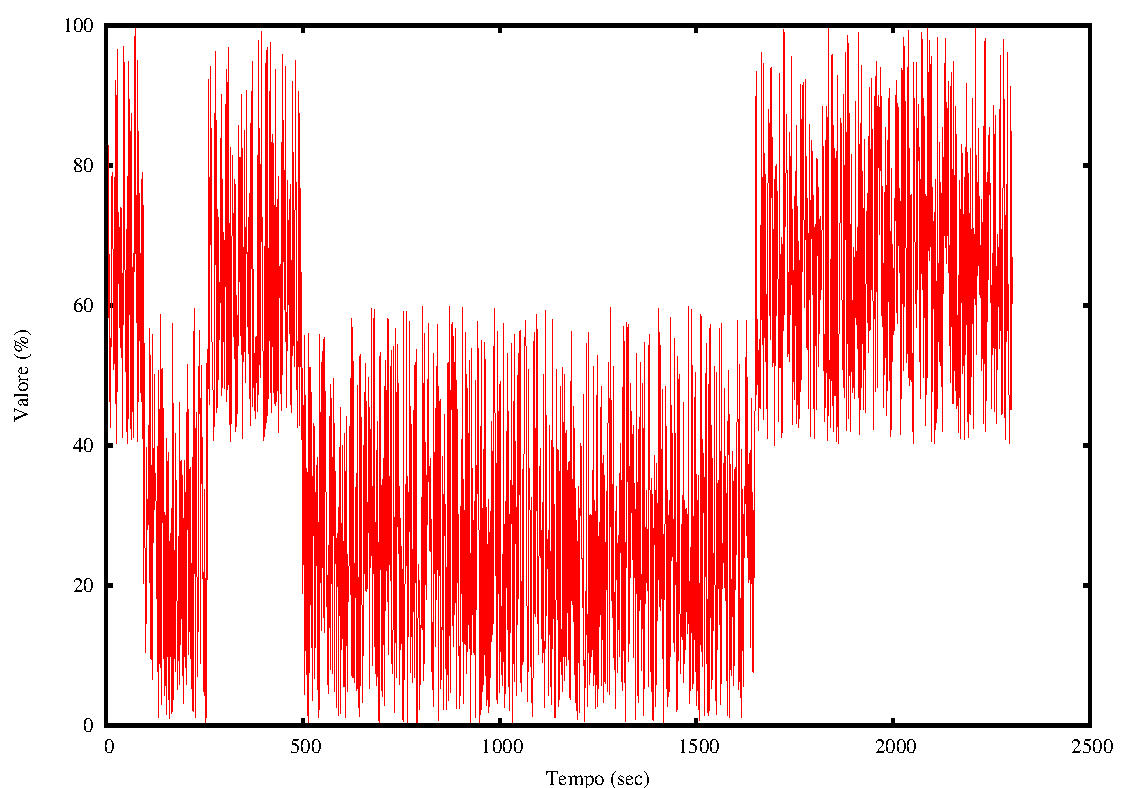
\includegraphics[scale=0.6]{etc/cpu1.pdf}
\caption{Cpu primo nodo}
\label{fig:cpu1}
\end{center}
\end{figure}
\begin{figure}[H]
\begin{center}
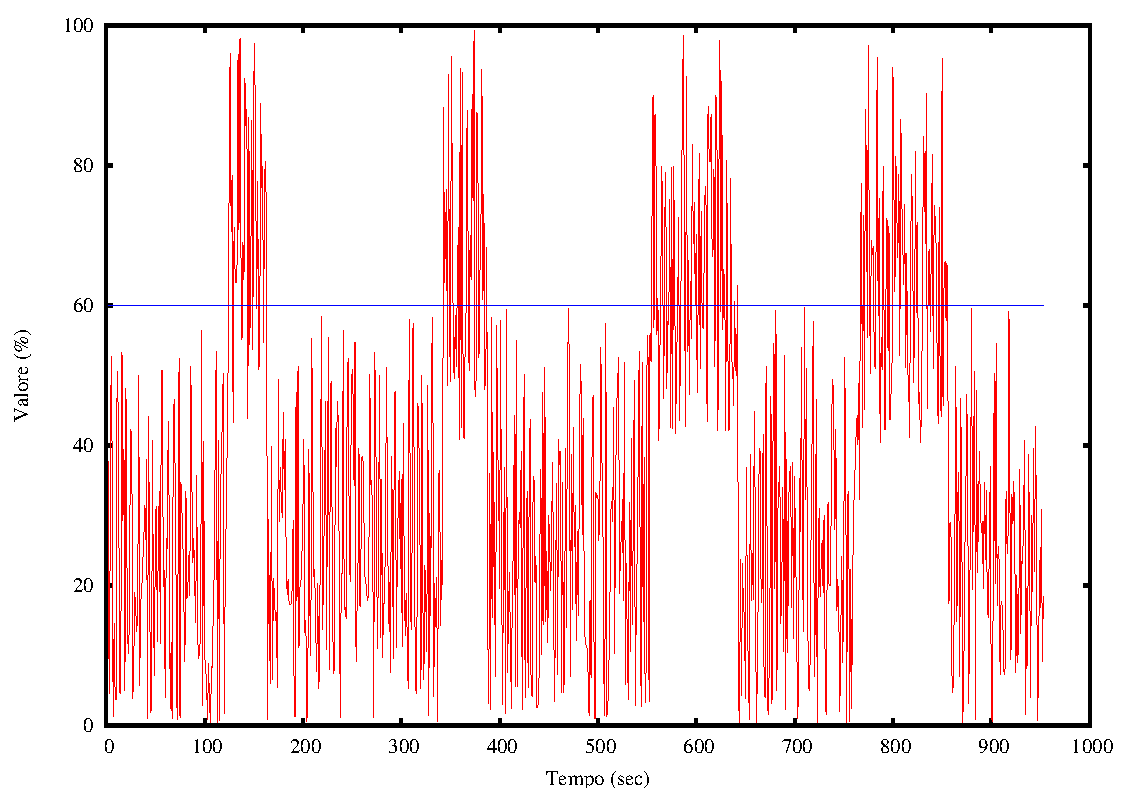
\includegraphics[scale=0.6]{etc/cpu2.pdf}
\caption{Cpu secondo nodo}
\label{fig:cpu2}
\end{center}
\end{figure}
\begin{figure}[H]
\begin{center}
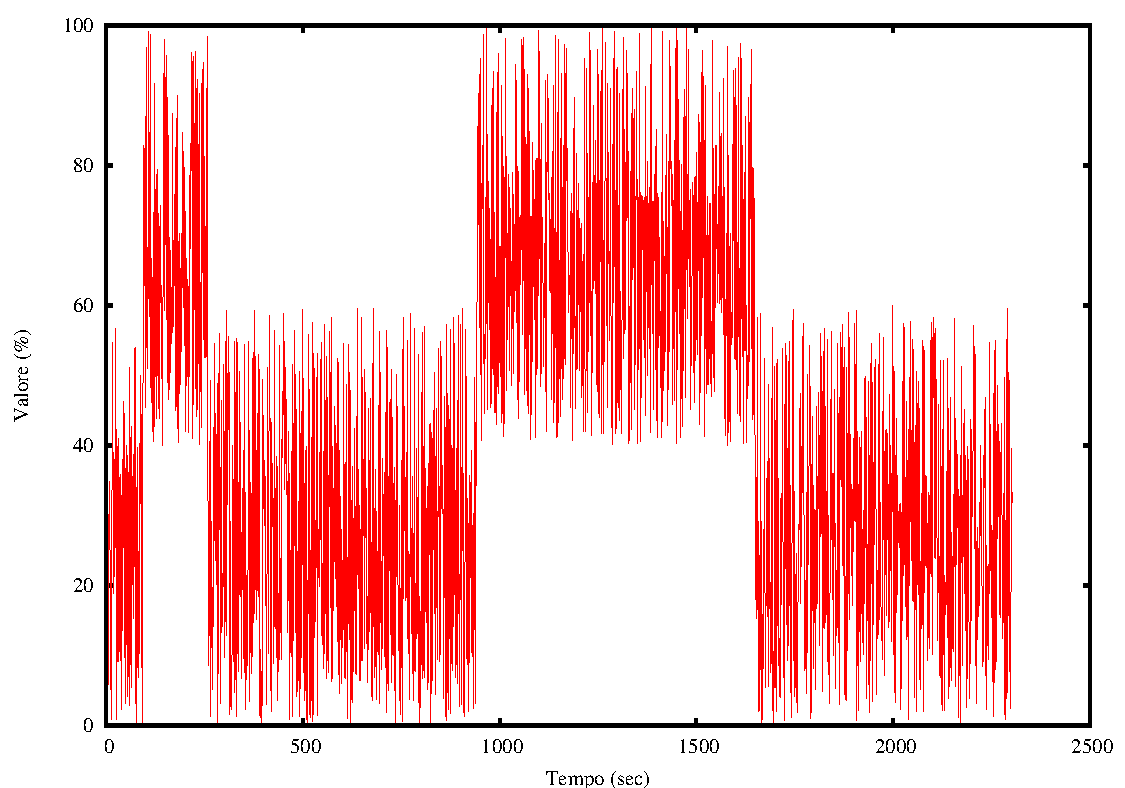
\includegraphics[scale=0.6]{etc/cpu3.pdf}
\caption{Cpu terzo nodo}
\label{fig:cpu3}
\end{center}
\end{figure}
\begin{figure}[H]
\begin{center}
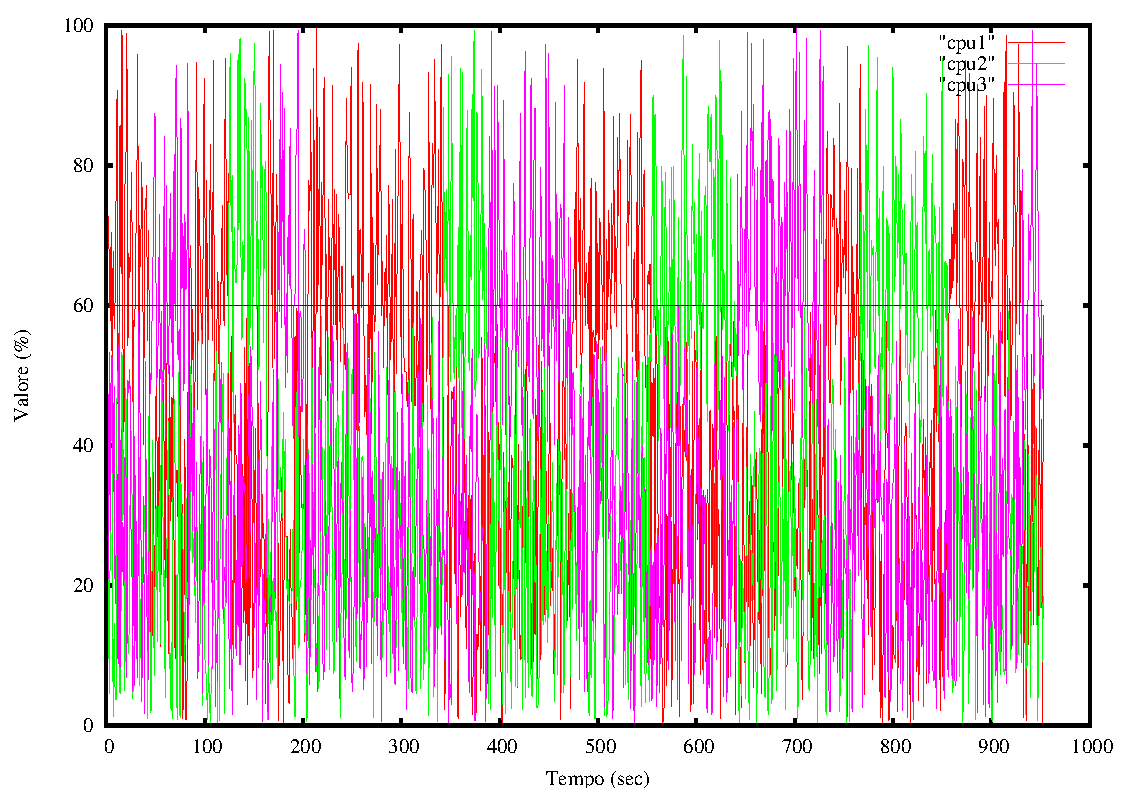
\includegraphics[scale=0.6]{etc/cpu.pdf}
\caption{Cpu tutti i nodi}
\label{fig:cpu}
\end{center}
\end{figure}
In tali grafici è presente una retta sul valore 60\% per distinguere il i nodi che hanno lo SC dagli altri, in particolare quando i valori si trovano oltre 60\% è presente lo SC sul nodo corrispondente. In presenza di una migrazione avviene un brusco cambiamento di carico, infatti si scende sotto il 60\%. Nella figura \ref{fig:cpu} sono graficati i tre nodi, questo crea confusione ma rende più semplicemente l'idea di come migri lo SC da un nodo ad un altro. Nello specifico si può notare che nella parte superiore al 60\% si trova sempre un nodo nel singono istante di tempo, questo è causato dalla presenza di un solo SC che si muove tra i nodi.

\subsection{Ram}
La ram ha una sensibilità come la cpu, infatti i valore vengono generati con le stesse formule. Dai grafici che seguono si possono notare i picchi di carico in corrispondenza delle migrazioni.
\begin{figure}[H]
\begin{center}
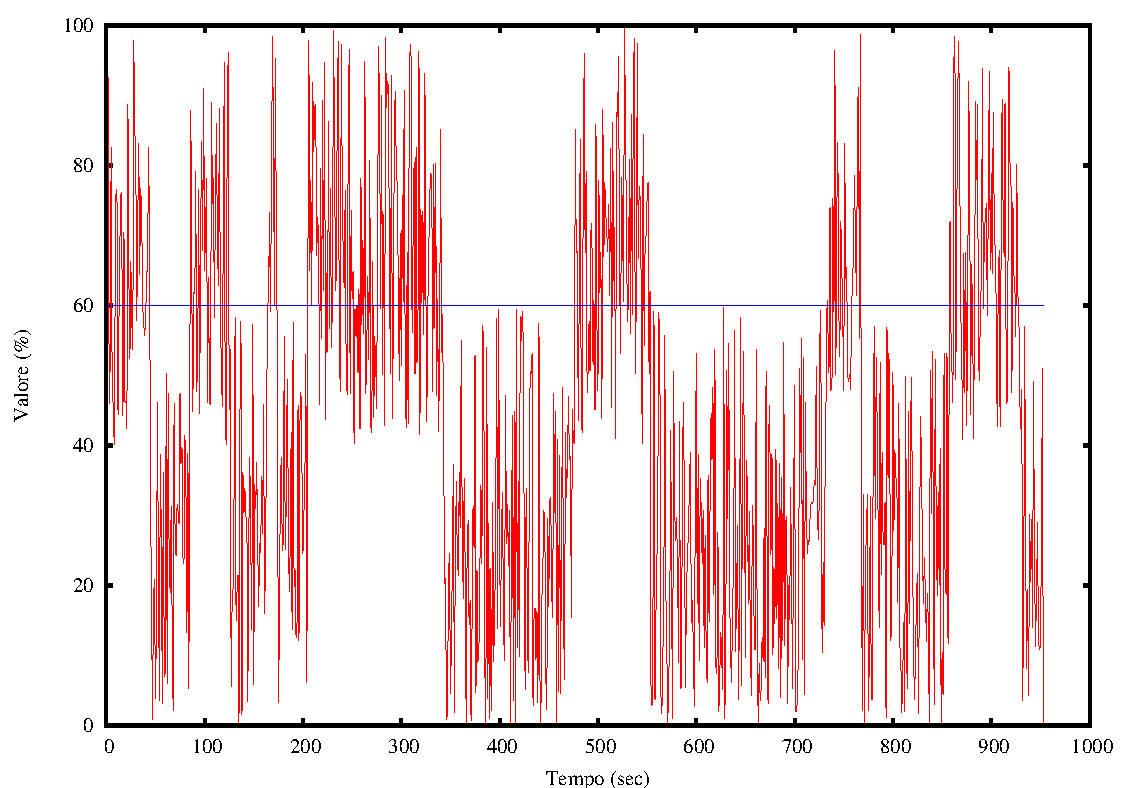
\includegraphics[scale=0.6]{etc/ram1.pdf}
\caption{Ram primo nodo}
\label{fig:ram1}
\end{center}
\end{figure}
\begin{figure}[H]
\begin{center}
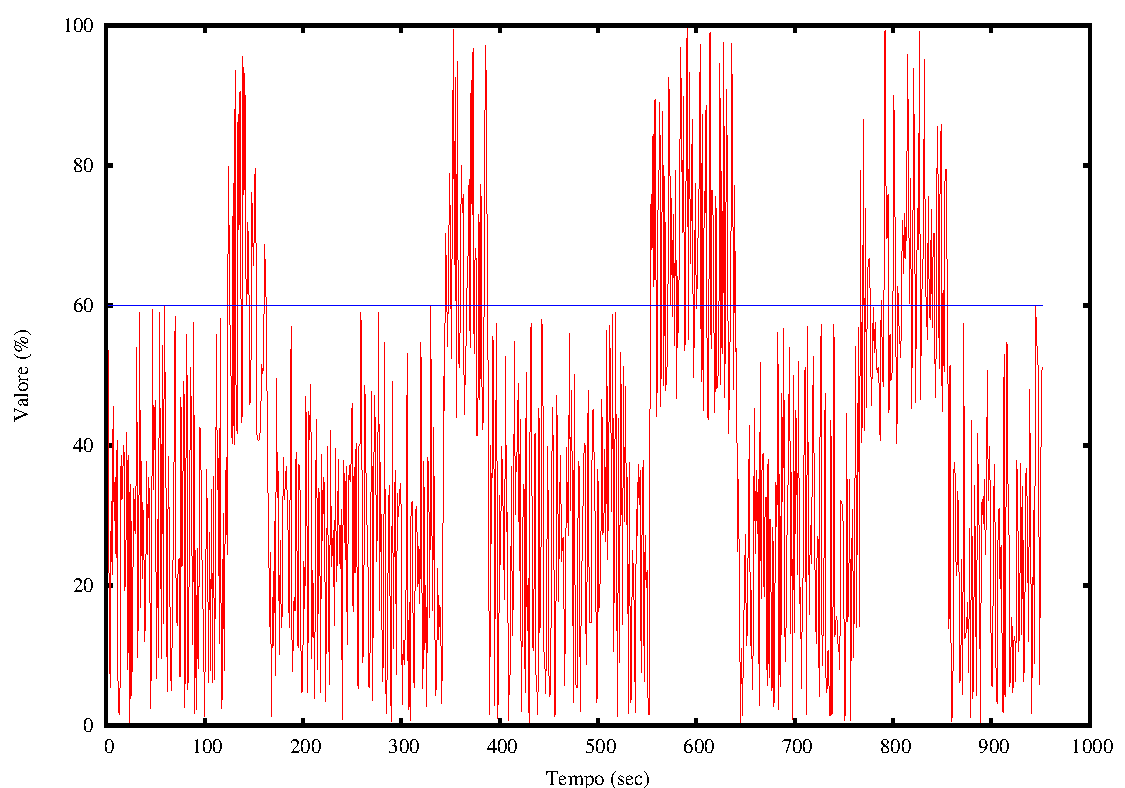
\includegraphics[scale=0.6]{etc/ram2.pdf}
\caption{Ram secondo nodo}
\label{fig:ram2}
\end{center}
\end{figure}
\begin{figure}[H]
\begin{center}
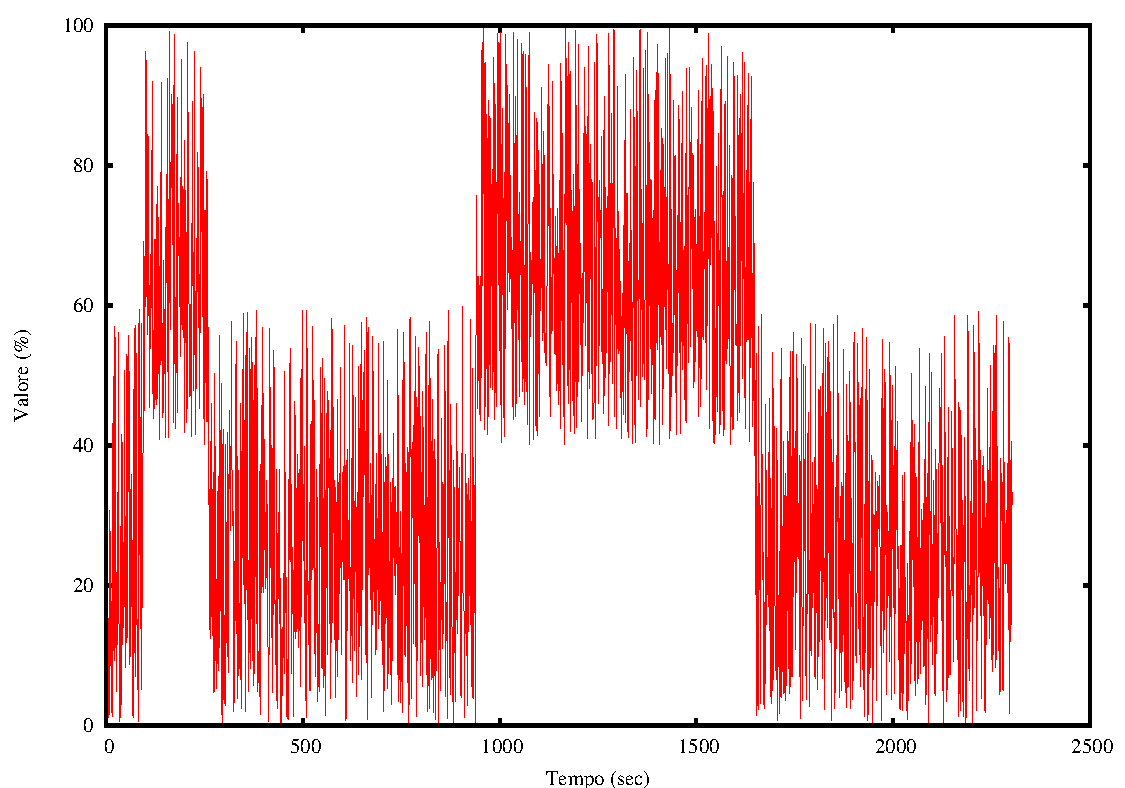
\includegraphics[scale=0.6]{etc/ram3.pdf}
\caption{Ram terzo nodo}
\label{fig:ram3}
\end{center}
\end{figure}
\begin{figure}[H]
\begin{center}
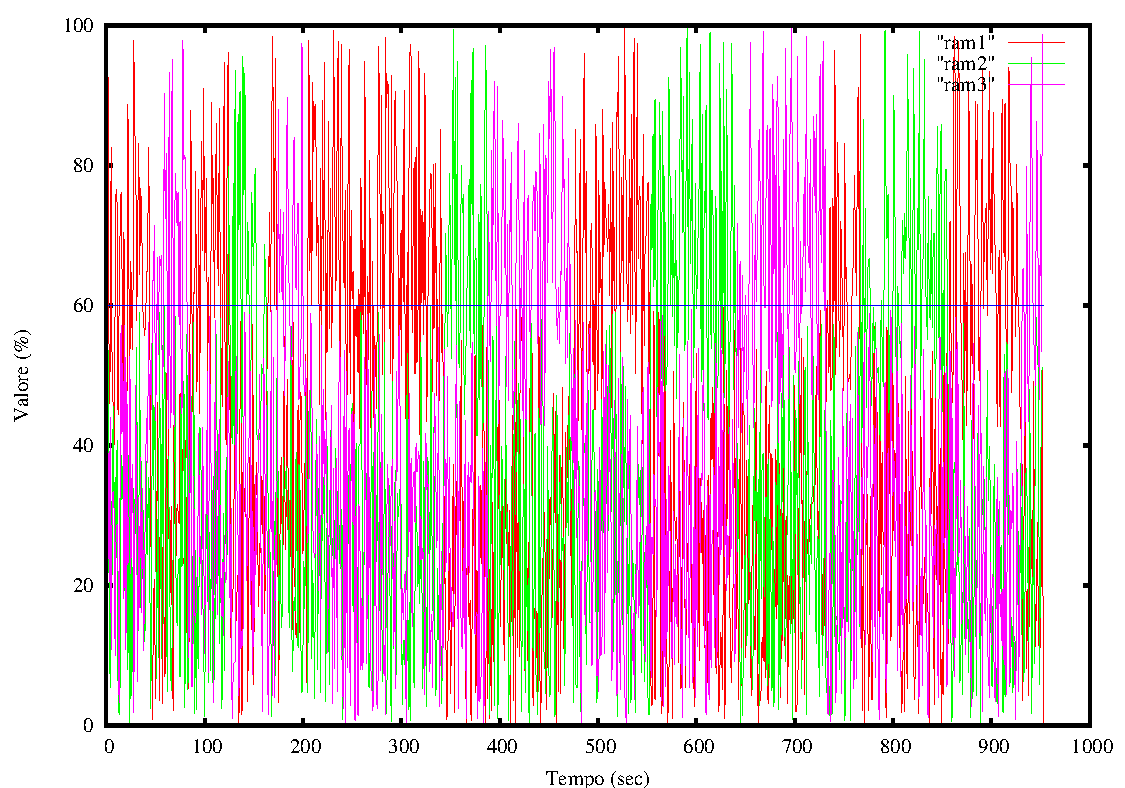
\includegraphics[scale=0.6]{etc/ram.pdf}
\caption{Ram tutti i nodi}
\label{fig:ram}
\end{center}
\end{figure}

\subsection{Memory}
La memoria è un parametro molto più dipendente dalle migrazioni, infatti in corrispondenza di esse si ha un incremento di utilizzazione costante ma non istantaneo. Dai grafici \ref{fig:memory1}, \ref{fig:memory2}, \ref{fig:memory3} e \ref{fig:memory} si può notare che quando i valori di memoria raggiungono la soglia dello 0 o del 100 si ha un picco di traffico verticale, questo non è dovuto alle migrazioni ma potrebbe essere associato, ad esempio, a generazioni di file temporanei da parte del nodo. In corrispondenza di incrementi di memoria costanti vuol dire che è presente lo SC, invece quando si hanno cali costanti si ha il contrario, ovvero lo SC è migrato su un altro nodo.
\begin{figure}[H]
\begin{center}
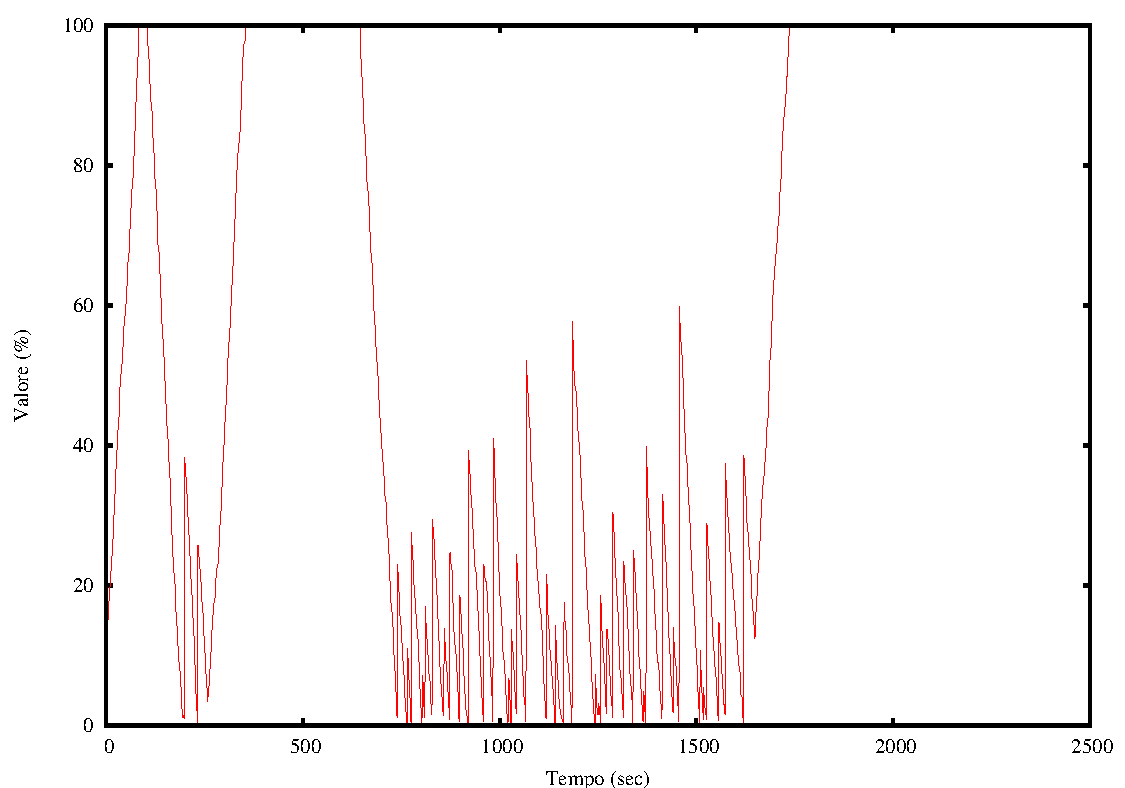
\includegraphics[scale=0.6]{etc/memory1.pdf}
\caption{Memory primo nodo}
\label{fig:memory1}
\end{center}
\end{figure}
\begin{figure}[H]
\begin{center}
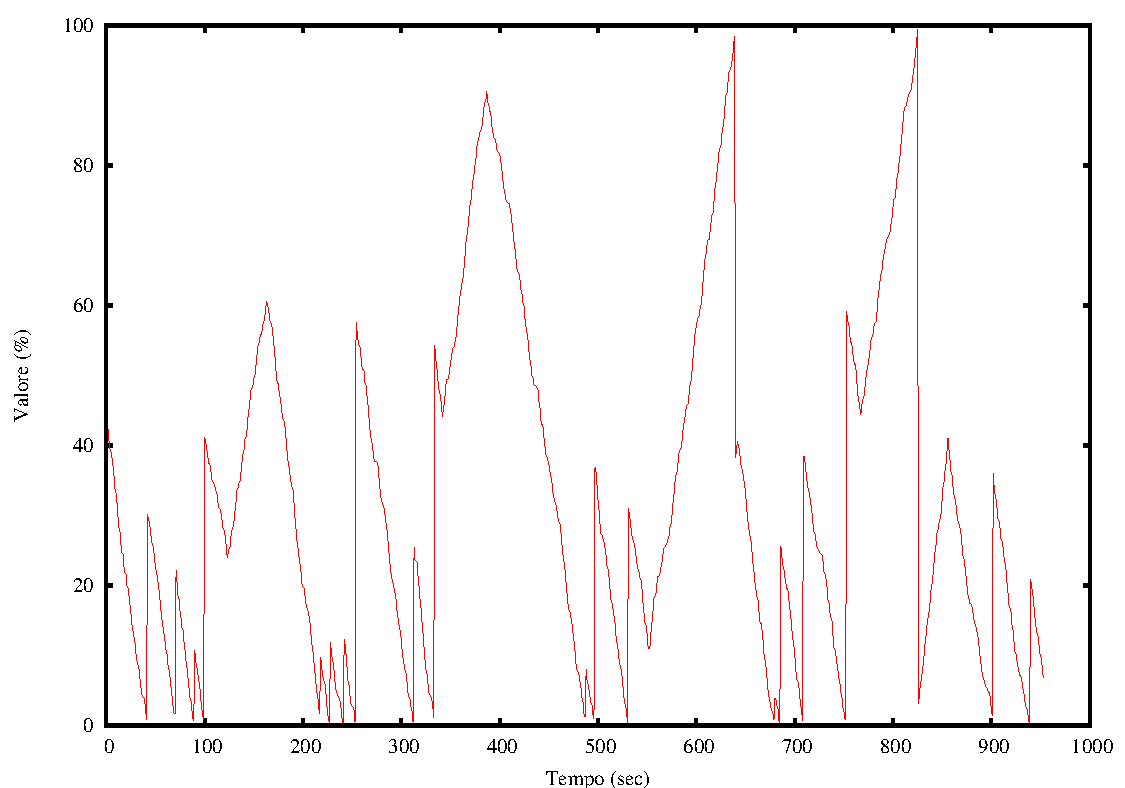
\includegraphics[scale=0.6]{etc/memory2.pdf}
\caption{Memory secondo nodo}
\label{fig:memory2}
\end{center}
\end{figure}
\begin{figure}[H]
\begin{center}
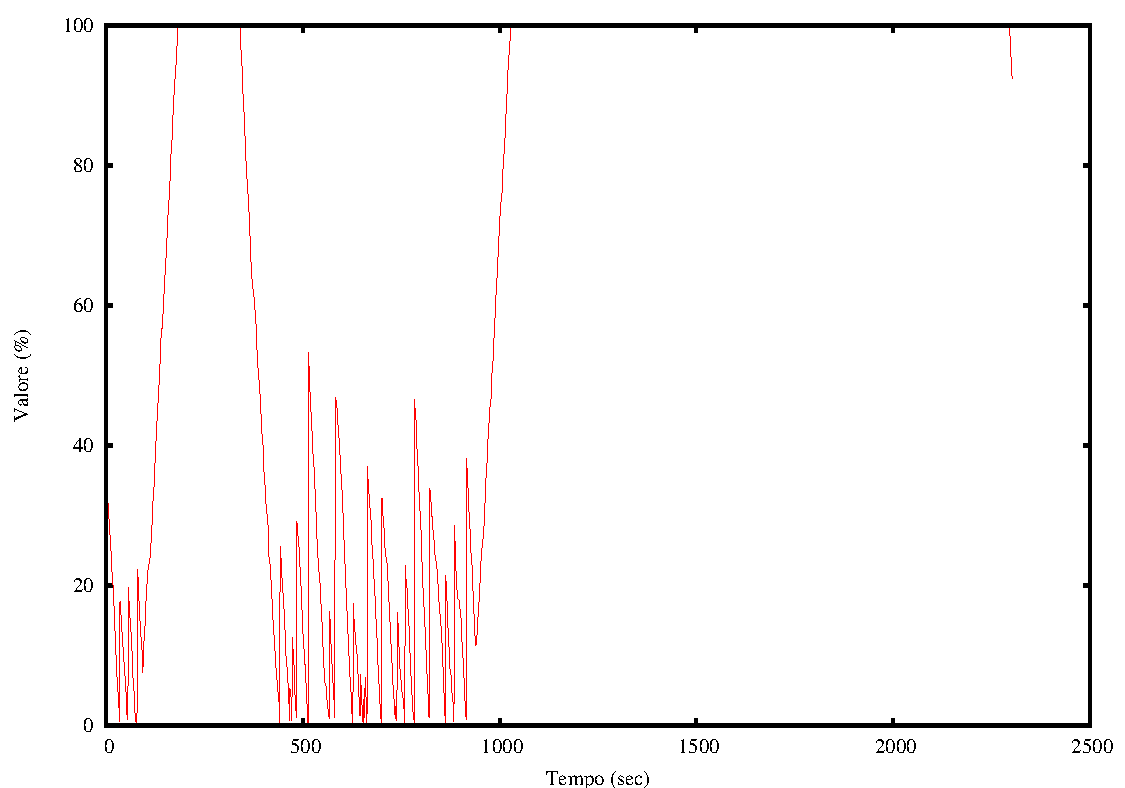
\includegraphics[scale=0.6]{etc/memory3.pdf}
\caption{Memory terzo nodo}
\label{fig:memory3}
\end{center}
\end{figure}
\begin{figure}[H]
\begin{center}
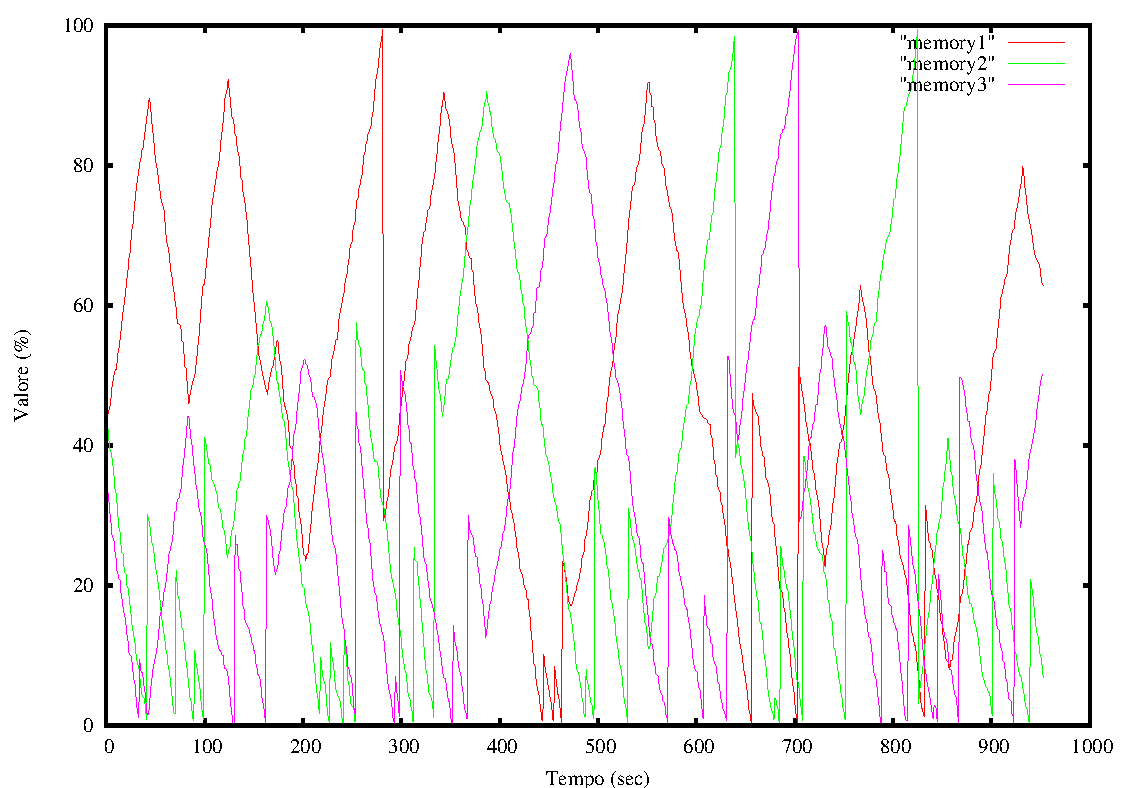
\includegraphics[scale=0.6]{etc/memory.pdf}
\caption{Memory tutti i nodi}
\label{fig:memory}
\end{center}
\end{figure}

\subsection{Energy}
L'energia è il parametro che varia più regolarmente in quanto dipende dal tipo di connessione e dalla presenza delle rete elettrica. Tale comportamento può essere notato dai grafici \ref{fig:energy1}, \ref{fig:energy2}, \ref{fig:energy3} e \ref{fig:energy}. In particolare in presenza dello SC su un nodo si ha un utilizzo di corrente maggiore, nello specifico se il nodo è connesso alla rete elettrica si ha un caricamento più lento, essendo parte dell'energia sprecata a causa dello SC; anche in caso di scollegamento dalla rete elettrica si ha uno spreco di energia maggiore causato dallo SC. Dalle figure si può anche notare che in corrispondenza del 10\% si ha un incremento di carica, essendo il nodo ricollegato alla rete elettrica, invece al raggiungimento del 100\% viene scollegato, considerando che il caricamento è completo. Un ulteriore particolare si può notare in figura \ref{fig:energy1}, in quanto il nodo è di tipo fisso e quindi con corrente sempre disponibile, infatti il valore di energia è sempre 100\%.
\begin{figure}[H]
\begin{center}
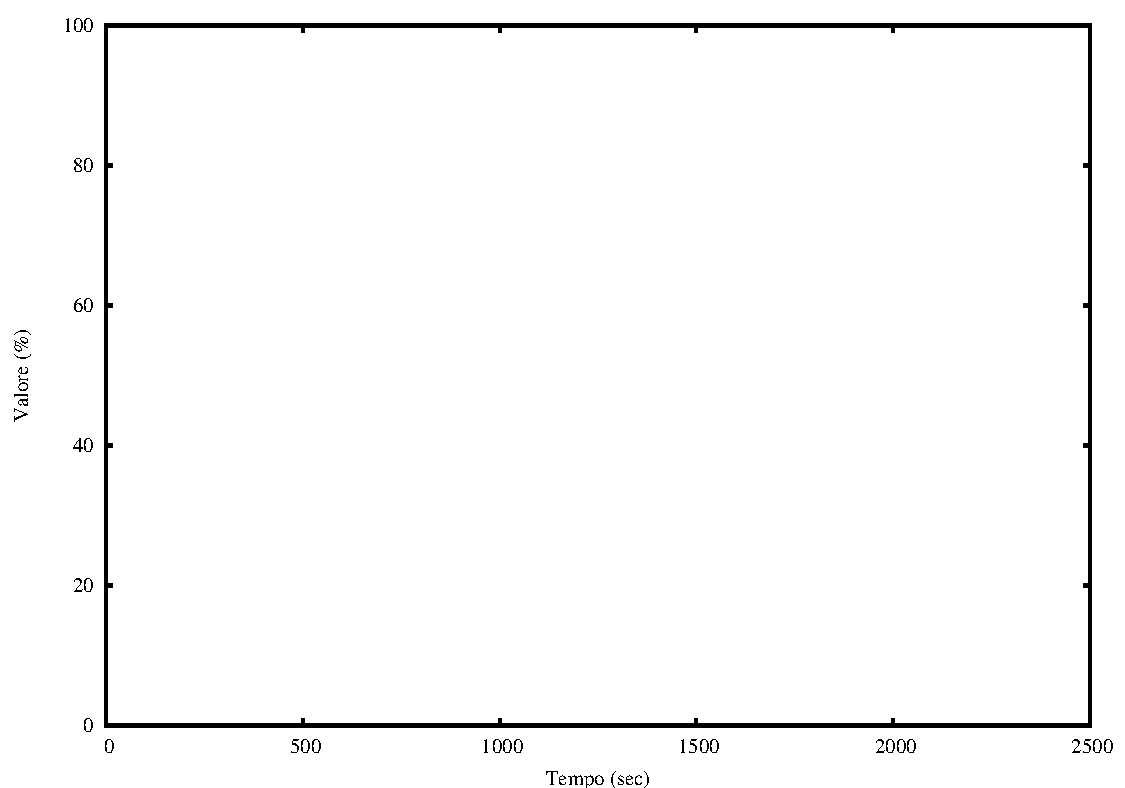
\includegraphics[scale=0.6]{etc/energy1.pdf}
\caption{Energy primo nodo}
\label{fig:energy1}
\end{center}
\end{figure}
\begin{figure}[H]
\begin{center}
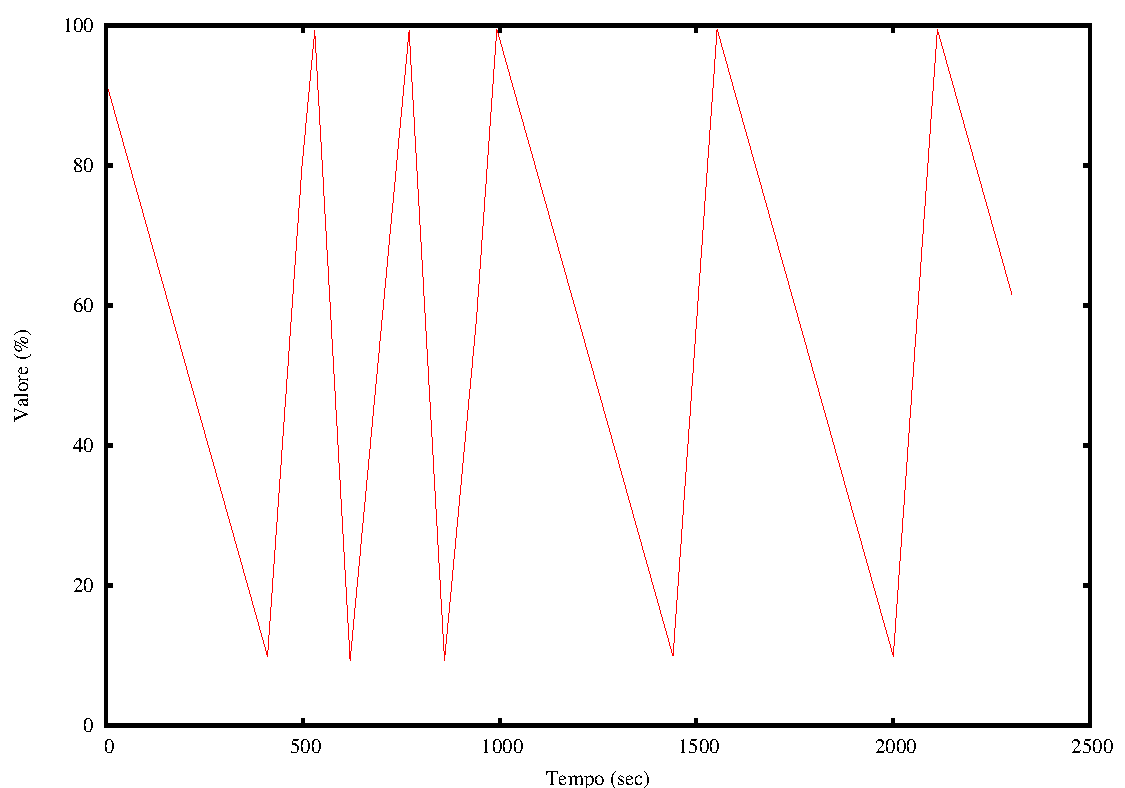
\includegraphics[scale=0.6]{etc/energy2.pdf}
\caption{Energy secondo nodo}
\label{fig:energy2}
\end{center}
\end{figure}
\begin{figure}[H]
\begin{center}
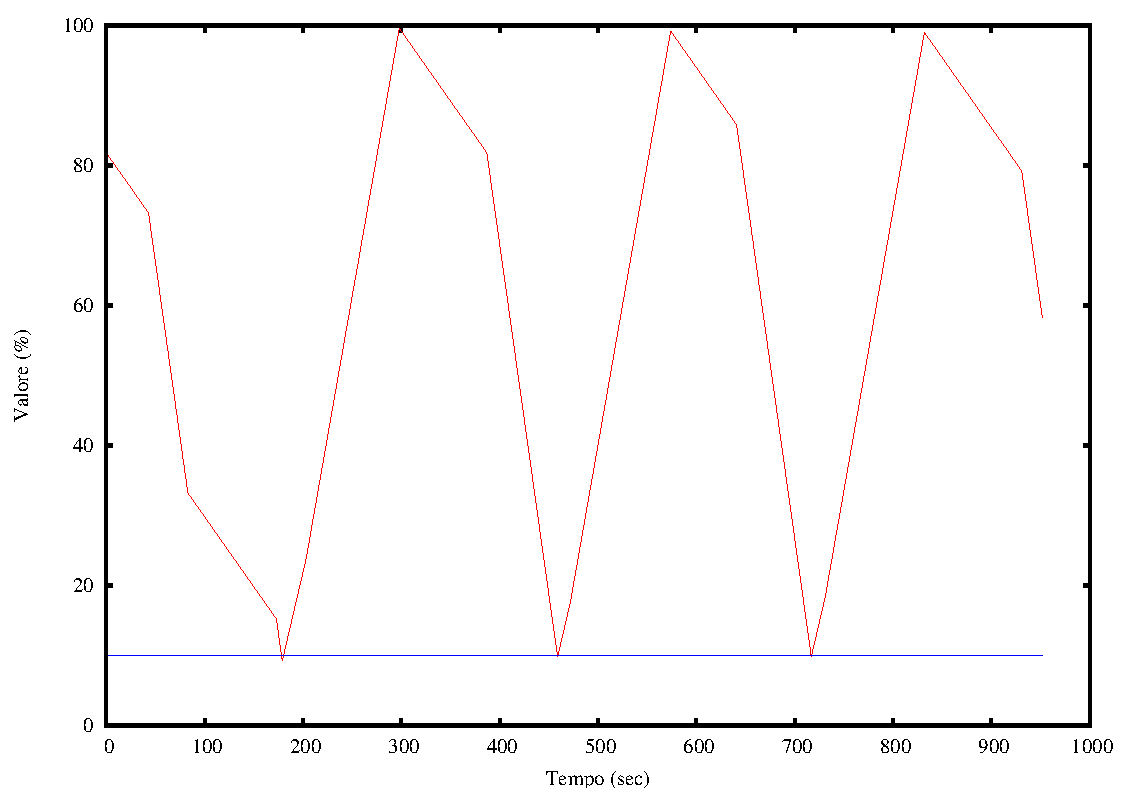
\includegraphics[scale=0.6]{etc/energy3.pdf}
\caption{Energy terzo nodo}
\label{fig:energy3}
\end{center}
\end{figure}
\begin{figure}[H]
\begin{center}
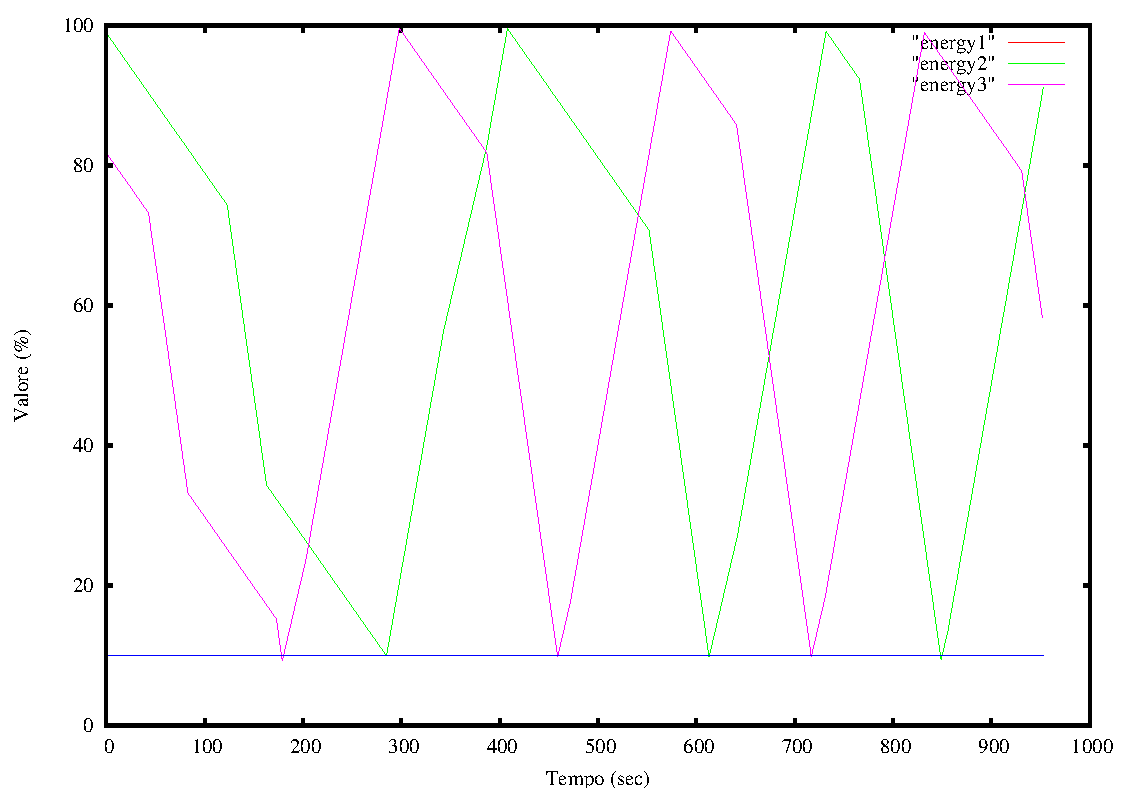
\includegraphics[scale=0.6]{etc/energy.pdf}
\caption{Energy tutti i nodi}
\label{fig:energy}
\end{center}
\end{figure}

\subsection{Latency}
Quest'ultimo valore generato dipendenze dalla presenza dell'SC, dal tipo di linea e dalla banda, come già riportato nel modello matematico. Nei seguenti grafici si possono vedere gli andamenti:
\begin{figure}[H]
\begin{center}
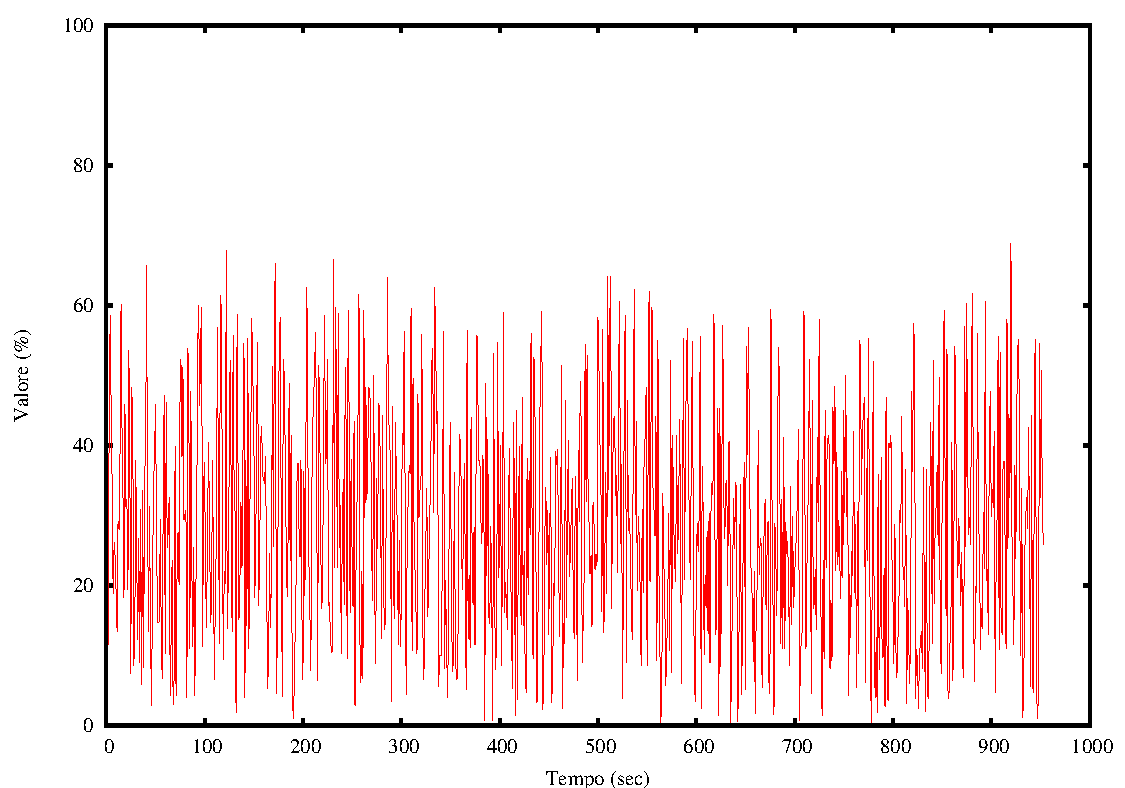
\includegraphics[scale=0.6]{etc/latency1.pdf}
\caption{Latency primo nodo}
\label{fig:latency1}
\end{center}
\end{figure}
\begin{figure}[H]
\begin{center}
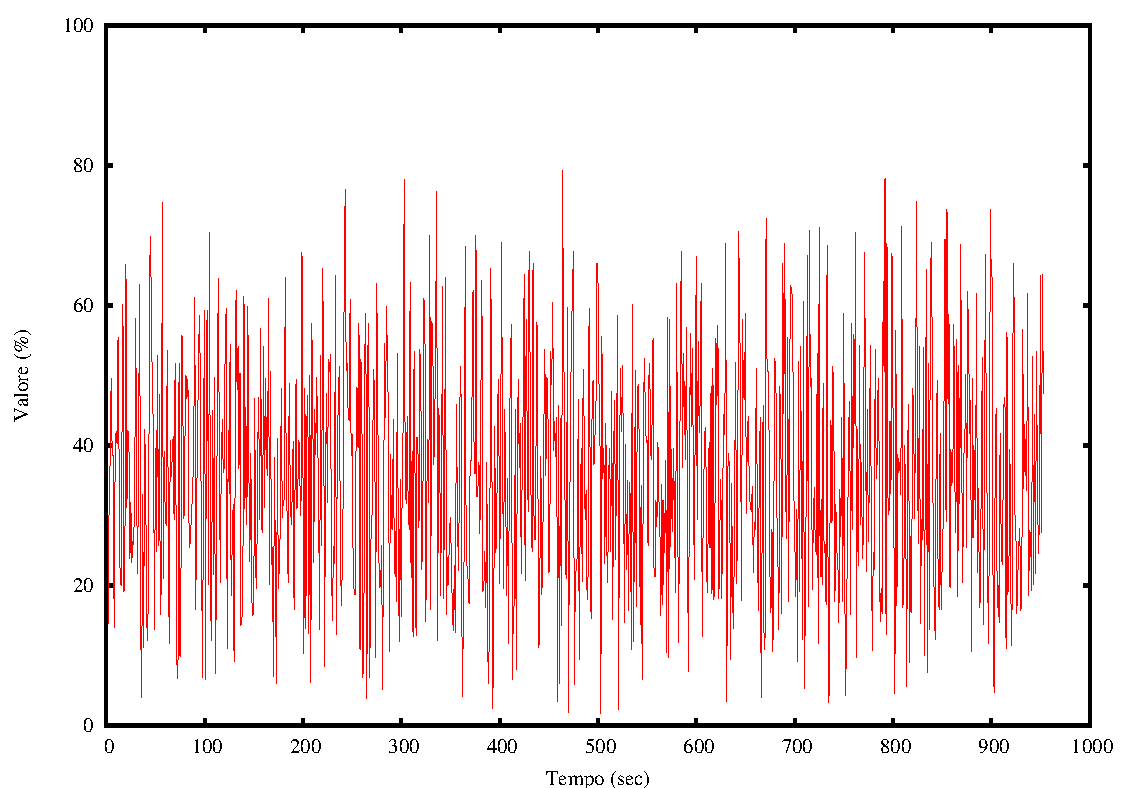
\includegraphics[scale=0.6]{etc/latency2.pdf}
\caption{Latency secondo nodo}
\label{fig:latency2}
\end{center}
\end{figure}
\begin{figure}[H]
\begin{center}
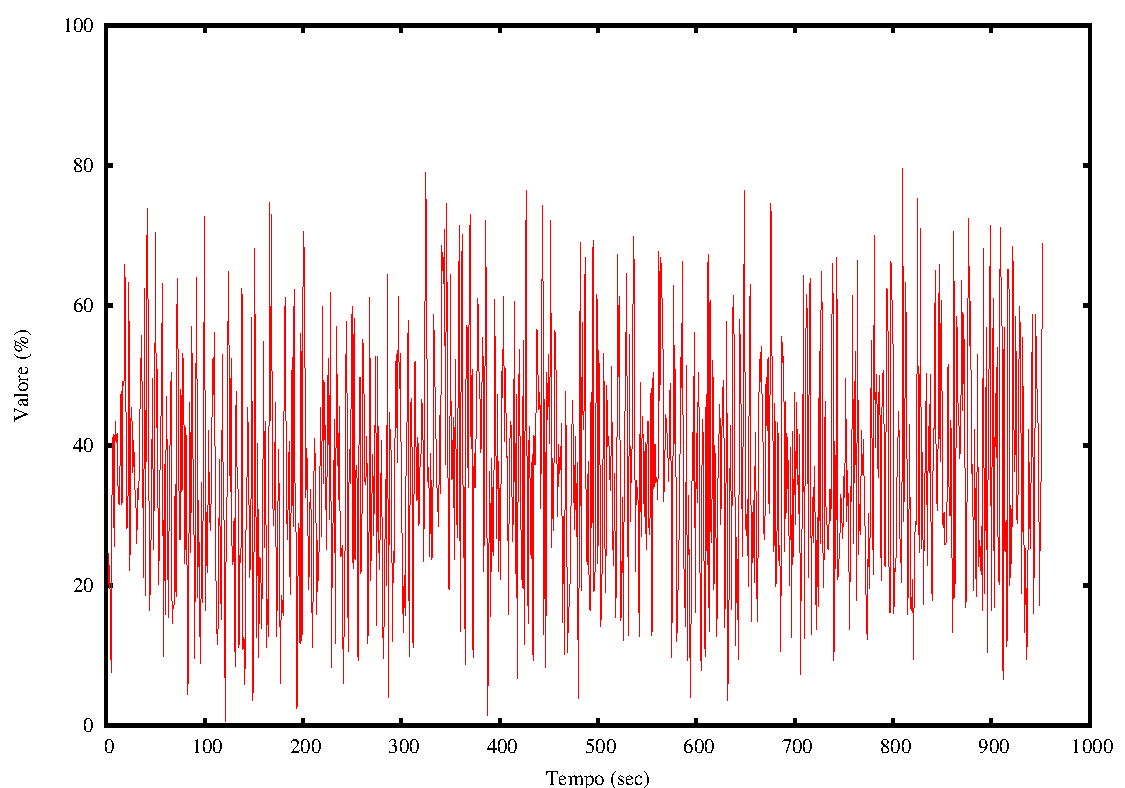
\includegraphics[scale=0.6]{etc/latency3.pdf}
\caption{Latency terzo nodo}
\label{fig:latency3}
\end{center}
\end{figure}
I valori in figura \ref{fig:latency1} è molto più basso rispetto ai valori in figura \ref{fig:latency2} e \ref{fig:latency3}, a causa della tipologia di connessione diversa.

\subsection{Reliability}
Questo valore è simile alla latenza ed anch'esso dipende fortemente dal tipo di connessione e dalla banda ma non dall'SC, il quale non influisce sulle caratteristiche della qualità della connessione. Nelle figure si può notare la differenza di valori tra il caso \ref{fig:reliability1} e i restanti.
\begin{figure}[H]
\begin{center}
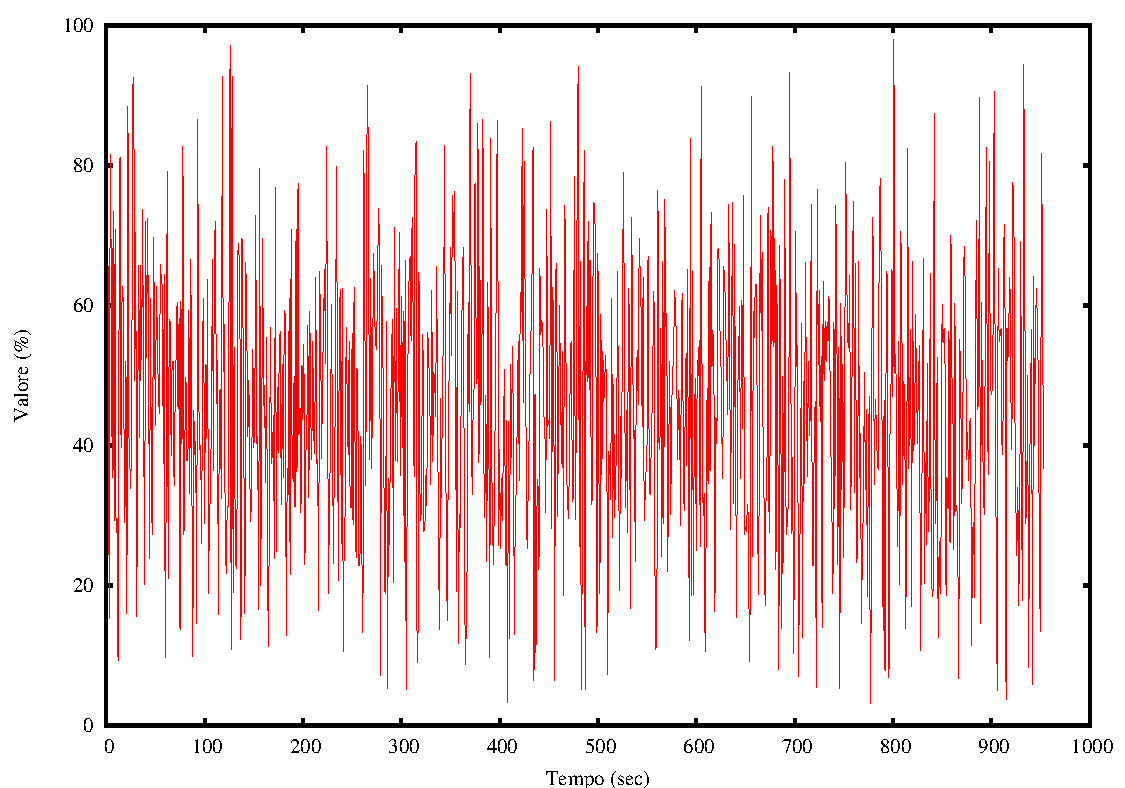
\includegraphics[scale=0.6]{etc/reliability1.pdf}
\caption{Reliability primo nodo}
\label{fig:reliability1}
\end{center}
\end{figure}
\begin{figure}[H]
\begin{center}
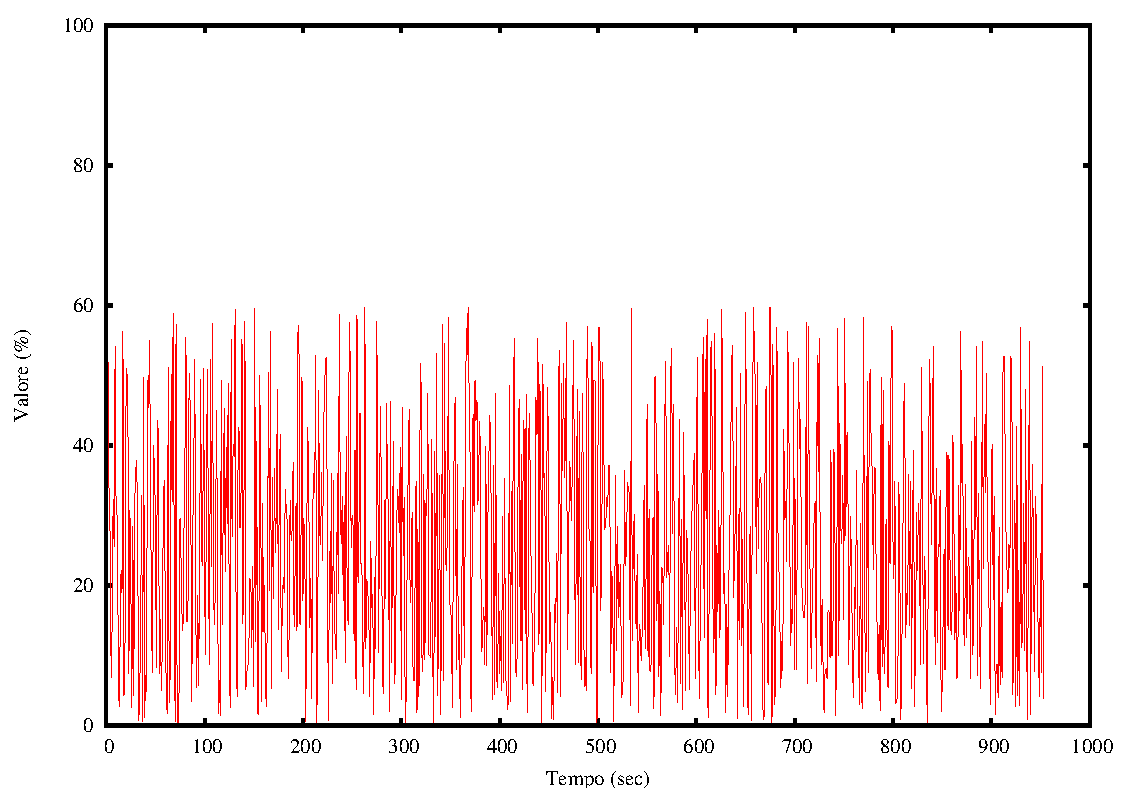
\includegraphics[scale=0.6]{etc/reliability2.pdf}
\caption{Reliability secondo nodo}
\label{fig:reliability2}
\end{center}
\end{figure}
\begin{figure}[H]
\begin{center}
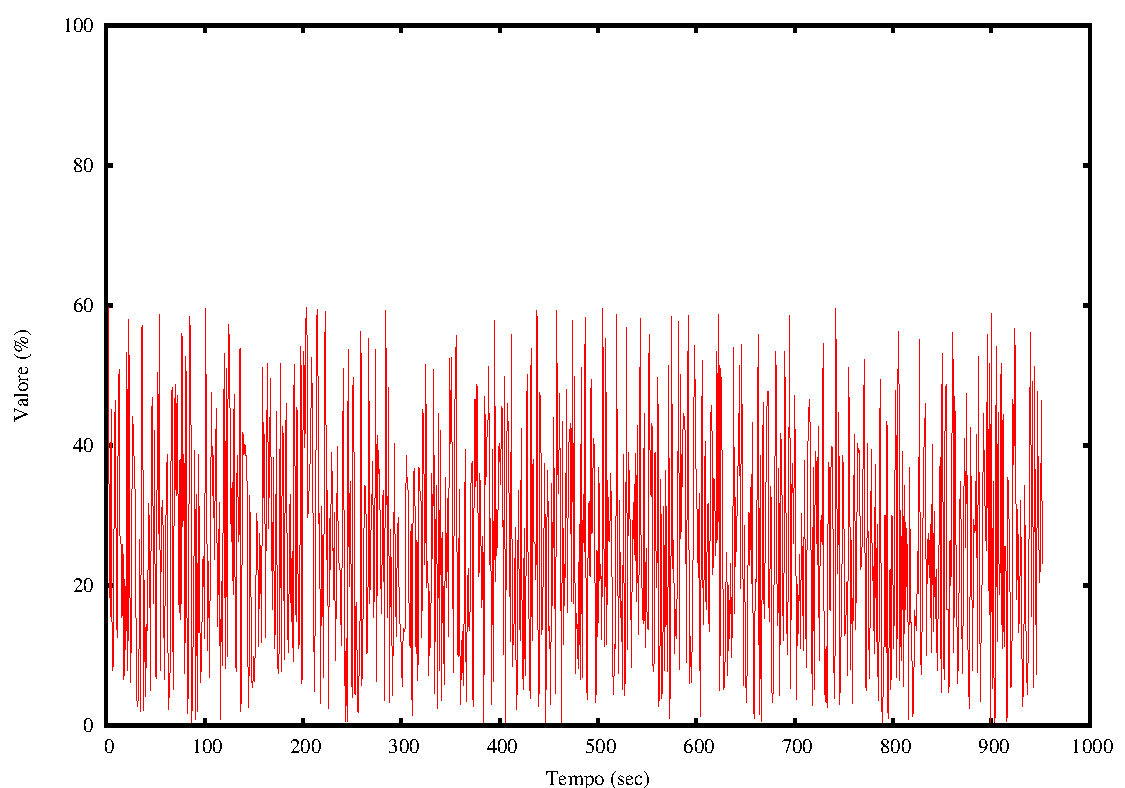
\includegraphics[scale=0.6]{etc/reliability3.pdf}
\caption{Reliability terzo nodo}
\label{fig:reliability3}
\end{center}
\end{figure}

\subsection{ReqInterval}
Quest'ultimo tipo di valore è strettamente casuale e può assumere valori tra lo 0\% e il 100\%.